\section{How TrustBazaar Closes Bikroy's Loopholes}
\label{sec:solution}

Sections~\ref{sec:history} and~\ref{sec:users} showed that Bikroy's weakness is not its app,
which users rate 4.3 out of 5~\cite{play_store}, but the \emph{transaction}: Bikroy controls who
may post an ad, but not the money, the handover or the dispute, and its terms say
so~\cite{bikroy_terms}. This section takes the six loopholes identified in
Section~\ref{sec:loopholes} and shows, one by one, which TrustBazaar feature closes each and
how. It then replays the documented scams against TrustBazaar's design, and ends with a direct
answer to the question of why anyone would use it. All TrustBazaar features cited here are
specified in our project proposal~\cite{proposal}.

\subsection{Loophole-to-feature mapping}

Table~\ref{tab:mapping} pairs each loophole with the feature that closes it, and
Figure~\ref{fig:mapping} shows the full picture: which features act as the primary fix for each
loophole and which support it. Escrow settlement alone is the primary fix for three of the six
loopholes (L2, L3 and L4), which is why the proposal treats it as part of the critical
path~\cite{proposal}.

\begin{table}[!tbp]
  \centering
  \small
  \caption{Each Bikroy loophole (Section~\ref{sec:loopholes}) and the TrustBazaar feature that
  closes it. Objective (Obj.) and acceptance-criterion numbers refer to the project
  proposal~\cite{proposal}; requirement identifiers (FR-KYC, FR-AUC) refer to version~2.0 of the
  project's SRS.}
  \label{tab:mapping}
  \begin{tabularx}{\textwidth}{@{}>{\raggedright\arraybackslash}p{2.9cm}
                                  >{\raggedright\arraybackslash}p{3.3cm} Y@{}}
    \toprule
    \textbf{Loophole on Bikroy} & \textbf{TrustBazaar feature} & \textbf{How it closes the gap} \\
    \midrule
    \textbf{L1 Weak identity}: phone OTP only; SIM cards cost Tk~350--500~\cite{fs_fraud,ds_muktagacha}
      & NID + selfie KYC before listing or buying (Obj.~1; FR-KYC-01--FR-KYC-11), with an AI pre-check of
        document quality and selfie match
      & The account is tied to a verified national identity, not a SIM card. A banned person
        cannot return by buying a new number. \\
    \addlinespace
    \textbf{L2 No payment protection}: money moves off-platform~\cite{bikroy_terms,bikroy_safety}
      & Escrow settlement through bKash, Nagad or card (Obj.~3)
      & The buyer pays into escrow; the seller is paid only after the buyer confirms receipt, or
        automatically after a fixed timeout. This is the principle Bangladesh Bank mandated for
        e-commerce in 2021~\cite{tbs_escrow}. \\
    \addlinespace
    \textbf{L3 Unsafe handover}: cash meetings enable robbery and note swaps~\cite{dt_2014,pa_2023}
      & System-arranged delivery (Obj.~4): a suggested safe public meetup point, or a courier
        at a system-quoted fare
      & No cash changes hands at the meeting, because payment is already in escrow. With nothing
        to count, there is nothing to swap. \\
    \addlinespace
    \textbf{L4 No recourse}: Bikroy is not a party; liability capped at
      BDT~6{,}700~\cite{bikroy_terms}
      & Dispute resolution by a platform operator while funds are still held
      & The dispute is raised before the money leaves escrow, so a refund is actually possible.
        Under the 2021 regime, Tk~2.14~bn still held in escrow could be returned to
        buyers~\cite{fe_refund}. \\
    \addlinespace
    \textbf{L5 No accountability record}: no verified history; no fraud data since 2014~\cite{dt_2014}
      & Ratings tied to completed transactions, and an auditable ledger of payment splits (Obj.~5)
      & Only someone who completed an escrow deal can leave a review, so reviews cannot be faked.
        Every payment split is recorded and inspectable in a dispute. \\
    \addlinespace
    \textbf{L6 No fair price discovery}: fixed prices and informal haggling only
      & Server-authoritative auction with proxy bids, reserve price, anti-sniping extension
        (Obj.~2; FR-AUC-01--FR-AUC-18) and bid-fraud detection
      & The server, not the client, decides the end time and the winner; a late bid extends the
        auction; suspicious bidding is flagged to the operator. \\
    \bottomrule
  \end{tabularx}
\end{table}

\begin{figure}[H]
  \centering
  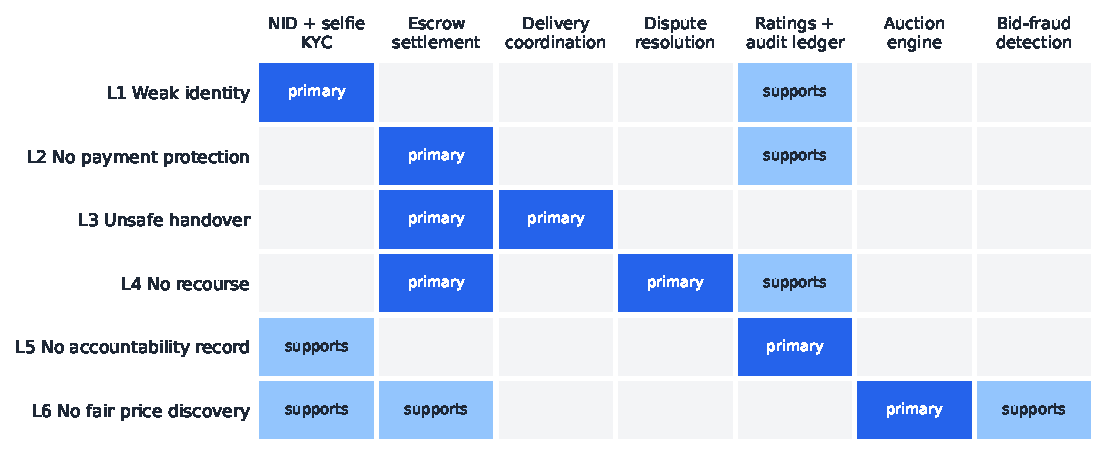
\includegraphics[width=\textwidth]{fig13_mapping.pdf}
  \caption{Which TrustBazaar feature addresses which Bikroy loophole. Dark cells: the feature is
  the primary fix; light cells: it supports the fix. Escrow settlement is the primary fix for
  three loopholes. Mapping derived from the TrustBazaar proposal~\cite{proposal}.}
  \label{fig:mapping}
\end{figure}

\subsection{Same transaction, different control}

Figure~\ref{fig:lifecycle} traced a used-goods deal through six stages and showed that Bikroy
has no control over the last three. Figure~\ref{fig:lifecycle_tb} draws the same six stages for
TrustBazaar. The difference is concentrated in the stages where the documented scams happen:
payment, handover and dispute.

\begin{figure}[H]
  \centering
  \resizebox{\textwidth}{!}{% Same six stages as Figure 11: Bikroy (top row) vs TrustBazaar (bottom row)
\begin{tikzpicture}[
  font=\footnotesize,
  stage/.style={draw=ink, fill=white, rounded corners=2pt, minimum width=2.15cm,
                minimum height=0.9cm, align=center, font=\footnotesize\bfseries},
  cover/.style={rounded corners=2pt, minimum width=2.15cm, minimum height=1.25cm,
                align=center, text width=2.0cm, font=\scriptsize},
  flow/.style={-{Stealth[length=2mm]}, draw=ink, thick}]

  \foreach \i/\name in {1/Identity, 2/Listing, 3/Contact \&\\negotiation,
                        4/Payment, 5/Handover, 6/Dispute \&\\recourse}{
    \node[stage] (s\i) at ({(\i-1)*2.45},0) {\name};
  }
  \foreach \a/\b in {1/2,2/3,3/4,4/5,5/6}{ \draw[flow] (s\a) -- (s\b); }

  % Bikroy row
  \node[cover, fill=partial!25] (b1) [below=0.35cm of s1] {Phone OTP only};
  \node[cover, fill=partial!25] (b2) [below=0.35cm of s2] {Ad review};
  \node[cover, fill=partial!25] (b3) [below=0.35cm of s3] {Chat or phone call};
  \node[cover, fill=bad!22]     (b4) [below=0.35cm of s4] {\textbf{None}:\\off-platform};
  \node[cover, fill=bad!22]     (b5) [below=0.35cm of s5] {\textbf{None}:\\cash meeting};
  \node[cover, fill=bad!22]     (b6) [below=0.35cm of s6] {\textbf{None}: liability\\$\le$ BDT 6,700};

  % TrustBazaar row
  \node[cover, fill=good!18] (t1) [below=0.25cm of b1] {NID + selfie KYC,\\operator review};
  \node[cover, fill=good!18] (t2) [below=0.25cm of b2] {Verified sellers only};
  \node[cover, fill=good!18] (t3) [below=0.25cm of b3] {In-app chat tied\\to the order};
  \node[cover, fill=good!18] (t4) [below=0.25cm of b4] {\textbf{Escrow}: held\\until receipt};
  \node[cover, fill=good!18] (t5) [below=0.25cm of b5] {Safe meetup point\\or booked courier;\\no cash};
  \node[cover, fill=good!18] (t6) [below=0.25cm of b6] {Operator dispute\\while funds\\are held};

  \node[anchor=east, font=\scriptsize\bfseries, text=muted, align=right]
    at ([xshift=-3pt]b1.west) {Bikroy};
  \node[anchor=east, font=\scriptsize\bfseries, text=good, align=right]
    at ([xshift=-3pt]t1.west) {Trust-\\Bazaar};
\end{tikzpicture}
}
  \caption{The six stages of a used-goods transaction, comparing Bikroy's control (top row,
  from Figure~\ref{fig:lifecycle}) with TrustBazaar's design (bottom row). Sources: Bikroy
  \cite{fs_fraud,ds_jiji,bikroy_terms}; TrustBazaar~\cite{proposal}.}
  \label{fig:lifecycle_tb}
\end{figure}

The core of this design is the escrow state machine in Figure~\ref{fig:escrow_states}. It
implements the proposal's third acceptance criterion: an escrow payment is never released
to a seller without either the buyer's explicit confirmation or a genuine timeout. It also
implements the fourth: a payment notice (webhook) that the provider delivers twice is never
processed twice~\cite{proposal}. Because the money is still held when a dispute is raised, a
refund is a database operation, not a police case.

\begin{figure}[H]
  \centering
  \resizebox{0.95\textwidth}{!}{% Escrow settlement state machine (TrustBazaar proposal, Objective 3 and Acceptance criterion 3)
\begin{tikzpicture}[
  font=\footnotesize, node distance=14mm and 17mm,
  st/.style={draw=#1, fill=#1!12, rounded corners=6pt, minimum height=1.0cm,
             text width=2.1cm, align=center, font=\scriptsize\bfseries},
  tr/.style={-{Stealth[length=2mm]}, thick, draw=ink},
  lab/.style={font=\scriptsize, inner sep=1.5pt, align=center}]

  \node[st=muted]                 (pay)  {Awaiting\\payment};
  \node[st=good, right=of pay]    (held) {Funds held\\in escrow};
  \node[st=good, right=of held]   (ship) {Item shipped or\\meetup set};
  \node[st=good, right=of ship]   (conf) {Buyer confirms\\receipt};
  \node[st=good, below=of conf]   (rel)  {Released\\to seller};
  \node[st=bad, below=of ship]    (disp) {Dispute\\raised};
  \node[st=muted, below=of held]  (dec)  {Operator\\decision};
  \node[st=bad, below=of pay]     (ref)  {Refunded\\to buyer};

  \draw[tr] (pay) -- node[lab, above]{buyer pays} (held);
  \draw[tr] (held) -- node[lab, above]{seller sends} (ship);
  \draw[tr] (ship) -- node[lab, above]{receives} (conf);
  \draw[tr] (conf) -- node[lab, right]{release} (rel);
  \draw[tr, densely dashed] (ship.south east) -- (rel.north west)
     node[lab, pos=0.45, right=1mm]{timeout,\\no reply};
  \draw[tr, bad] (ship) -- node[lab, left, text=bad]{buyer\\objects} (disp);
  \draw[tr] (disp) -- node[lab, above]{evidence +\\ledger} (dec);
  \draw[tr] (dec) -- node[lab, above]{buyer\\right} (ref);
  \draw[tr] (dec.south) to[out=-35, in=-145] node[lab, below, pos=0.5]{seller right} (rel.south);

  \node[font=\scriptsize\itshape, text=muted, align=left, anchor=north west, text width=13cm]
    at ([yshift=-17mm]ref.south west)
    {Money leaves escrow only after the buyer confirms, after the timeout expires, or by an
     operator decision; never on the seller's word alone. A payment notice that the provider
     sends twice is processed only once.};
\end{tikzpicture}
}
  \caption{TrustBazaar's escrow settlement as a state machine. Money can leave escrow by only
  three routes: buyer confirmation, an expired timeout, or an operator's dispute decision.
  Based on Objective~3 and Acceptance criteria~3--4 of the proposal~\cite{proposal}.}
  \label{fig:escrow_states}
\end{figure}

\subsection{Replaying the documented scams}

Table~\ref{tab:replay} takes each scam pattern documented in Section~\ref{sec:users}
(Table~\ref{tab:scams}) and shows where TrustBazaar's design stops it.

\begin{table}[H]
  \centering
  \small
  \caption{The scam patterns documented on Bikroy, replayed against TrustBazaar's design.}
  \label{tab:replay}
  \begin{tabularx}{\textwidth}{@{}>{\raggedright\arraybackslash}p{4.0cm} Y@{}}
    \toprule
    \textbf{Documented scam} & \textbf{What happens on TrustBazaar} \\
    \midrule
    Fake seller, advance payment (Muktagacha)~\cite{ds_muktagacha}
      & Each SIM-bought account would still need a real NID and selfie to list, blocking the
        scam at the start. Even if a fake listing slipped through, the buyer's money sits in
        escrow, so non-delivery leads to a refund instead of a loss. \\
    \addlinespace
    Lure and robbery (2014)~\cite{dt_2014}
      & The system suggests a public meetup point, or the buyer uses a courier and never meets
        the seller. Both parties' verified identities are on record. \\
    \addlinespace
    Counterfeit or swapped cash (2023 iPhone case)~\cite{pa_2023}
      & No cash at the meeting: payment is already held in escrow. \\
    \addlinespace
    Fake or replica goods~\cite{fs_fraud}
      & The buyer inspects the item and can raise a dispute before any money is released. \\
    \addlinespace
    Fake inquiries after paid promotion~\cite{trustpilot}
      & TrustBazaar's revenue is a commission on \emph{completed} sales~\cite{proposal}, not a
        charge per click. The platform earns only when a real deal happens, unlike the
        pay-per-click model Bikroy is moving to under Jiji~\cite{fs_jiji}. \\
    \bottomrule
  \end{tabularx}
\end{table}

\subsection{Market position: what TrustBazaar offers that incumbents do not}

The mapping above implies five points about where TrustBazaar sits in the market.

\begin{enumerate}[label=\textbf{\arabic*.}]
  \item \textbf{It targets a slice of the market, not the whole of it.} Most of Bikroy's transaction value is in
  cars and property~\cite{fs_jiji}, but most of its ads are used phones, electronics and
  household goods (Section~\ref{sec:catalogue}). TrustBazaar is designed for that
  individual-to-individual resale of used goods~\cite{proposal}, the part of the market where
  the documented scams cluster~\cite{ds_muktagacha,pa_2023} and where a buyer has no way to
  verify a stranger.

  \item \textbf{It differs in kind from every previous challenger.} OLX, Ekhanei and Jiji all ran
  listing boards~\cite{fs_ekhanei,intellinews}. None of them competed on the transaction
  itself. TrustBazaar is a different kind of product: a settlement platform, not a
  classifieds board.

  \item \textbf{It applies a protection Bangladesh has already adopted.} After the Evaly failures, the
  state required escrow for e-commerce payments~\cite{tbs_escrow}, and money still held in
  escrow was returned to buyers~\cite{fe_refund}. That regime never reached person-to-person
  resale (Section~\ref{sec:users}). TrustBazaar applies a protection the state has already
  validated to the part of the market it misses.

  \item \textbf{It suits the individual sellers Bikroy is moving away from.} Under Jiji, pay-per-click
  bidding favours sellers with marketing budgets~\cite{fs_jiji}. A fee charged only on completed
  deals better suits someone selling one used phone.

  \item \textbf{It offers what Facebook groups do not.} They have no verification, no payment handling
  and no record of who committed to buy~\cite{proposal}. For a buyer about to send a large sum to a
  stranger, TrustBazaar's offer is simple: the money does not move until the buyer has
  the item.
\end{enumerate}

\subsection{Limits and risks}

The design does not remove every barrier to adoption. Table~\ref{tab:limits} lists the main
risks and how TrustBazaar's design responds to each.

\begin{table}[H]
  \centering
  \small
  \caption{Main risks to TrustBazaar's adoption and the design response.}
  \label{tab:limits}
  \begin{tabularx}{\textwidth}{@{}>{\raggedright\arraybackslash}p{2.4cm}
                                  >{\raggedright\arraybackslash}p{4.6cm} Y@{}}
    \toprule
    \textbf{Risk} & \textbf{Why it is real} & \textbf{Design response} \\
    \midrule
    Network effect
      & Bikroy has about 400{,}000 monthly buyers and 100{,}000 monthly sellers~\cite{fs_jiji};
        a new platform starts with none.
      & This is the main open risk and is not solved by design alone. The project's aim is to
        demonstrate that the trust mechanisms work correctly, not to reach market
        scale~\cite{proposal}. \\
    \addlinespace
    KYC friction
      & Users already complain about Bikroy's manual checks~\cite{trustpilot}.
      & KYC is done once, not per ad. It gives the user something back (escrow protection and
        a verified badge) rather than being a cost with no return. \\
    \addlinespace
    Seller cash-flow delay
      & Escrow holds the money until the buyer confirms.
      & An automatic release timeout means a silent buyer cannot hold the funds
        indefinitely~\cite{proposal}. \\
    \addlinespace
    Regulation
      & Holding customers' money requires a licensed payment partner.
      & The academic build uses sandbox and test-mode integrations, stated openly~\cite{proposal}.
        A real launch would route funds through a licensed gateway's escrow service, the model
        the 2021 Bangladesh Bank rule uses~\cite{tbs_escrow}. \\
    \addlinespace
    Fees
      & Buyers and sellers may resist paying a commission.
      & The fee is charged only on a successful, protected deal, set against the documented
        cost of being scammed. \\
    \bottomrule
  \end{tabularx}
\end{table}

\subsection{Summary}

Bikroy has led the market since 2012 without being challenged on what it does not do. It
is a listing board that leaves payment, handover and disputes to chance, and its own terms say
so~\cite{bikroy_terms}. TrustBazaar does not compete on the number of ads. It closes the six
loopholes that Bikroy, Facebook groups and the 2021 escrow rule all leave open for individual
resale. Its value proposition is therefore not scale but safety: it is designed to protect
exactly the deals that Bikroy's terms decline responsibility for.
